
%----------------------------------------------------------------%%----------------------------------------------------------------%

\chapter{Changes in the Demographic Profile of Hospital Patients}

%----------------------------------------------------------------%%----------------------------------------------------------------%

\vspace{0.5in}

\textbf{Paper:}
\textsc{\underline{Andreas H\"ohn}, Anna Oksuzyan, Rune Lindahl-Jacobsen, 
	    Roland Rau, and Kaare Christensen:} Preparing for the future: The 
	    changing demographic composition of hospital patients in Denmark 
	    between 2014 and 2050. \textbf{\textit{Submitted to a peer-reviewed journal}} 

%----------------------------------------------------------------%%----------------------------------------------------------------%

\newpage

\section{Abstract}
% BACKGROUND %
\textbf{Background:} Preparing the healthcare workforce for 
population aging is a public health challenge, especially as 
medical students tend to avoid the field of geriatrics. We 
describe the current demographic profile of hospital care use 
in Denmark, project changes up to 2050, and interpret this in 
the light of the attitudes of students in the healthcare 
workforce.\\ 
% METHODS %
\textbf{Methods:} The Danish population in 2014 (N=5.63 million) 
was followed up for inpatient and emergency admissions recorded 
in Danish hospitals in 2014 using population-based registers. We 
combined age and sex-specific patterns of hospital care use in 
2014 with official population estimates to forecast the profile 
of hospital days up to 2050 with respect to age and sex.\\ 
% RESULTS %
\textbf{Results:} The total number of hospital days per year is 
projected to increase by 47\% between 2014 and 2050, from 3.75 
to 5.51 million days. While small changes are projected among 
the population aged 0-69, the largest change is projected to 
occur among the population aged 70+. The 2014 levels were 0.77 and 
0.84 million days for men and women aged 70+, respectively. By 
2050, these levels are projected to have reached 1.76 and 1.63 
million days. Whereas the population aged 70+ accounted for 42.9\% 
of all days in 2014, their contribution is projected to increase 
to 61.4\% by 2050.\\
% CONCLUSION %
\textbf{Conclusion:} Specific attention should be given to the 
education of the future healthcare workforce, as negative 
stereotypes and prejudice towards older individuals are important 
factors discouraging medical students and student nurses from 
joining the field of geriatrics.\\


%----------------------------------------------------------------%%----------------------------------------------------------------%


\newpage


%%% Introduction %%%
\section{Introduction}

Decreasing mortality trends in high and middle income countries will 
rapidly increase the population share of older individuals within the 
next few decades.\citep{kontis2017future} Currently, in these countries, 
approximately one person in six is aged 65 or older. By 2050, it is projected 
that the number of people aged 65+ will have almost doubled within these 
countries, and that nearly one in three will be 65 or older.\citep{desa2017world}
As the prevalence of non-communicable diseases increases with age - including 
cancers,\citep{campisi2013aging} circulatory diseases,\citep{leening2014sex} 
and dementia\citep{rasmussen2018absolute} - population aging presents new 
challenges for healthcare systems, including hospital settings.\citep{beard2015towards,
pallin2014us} Preparing the medical workforce for the changing demographic 
profile of patients has been identified as one of these challenges.\citep{bodenheimer2009confronting} 
Efficient delivery of high-quality care requires an adequate supply of 
well-trained health workers to meet the needs of patients. Already, a number 
of countries have reported substantial shortfalls in skilled medical workers.\citep{darzi2016global}

A growing body of literature has reported that medical students and 
student nurses tend to have negative attitudes towards older individuals.\citep{samra2015medical,
kusumastuti2017contact,fisher2018pejorative} Working with older patients has 
often been described as a burden and as less satisfying than working with 
younger patients. Negative attitudes towards the elderly have been shown to 
be important predictors for the quality of care and treatment,\citep{wilson2018medical} 
and are one main reason why young medical professionals tend to avoid the 
field of geriatrics.\citep{hughes2008medical} Recent studies suggest that 
medical students are not aware of who their future patients will be.\citep{kusumastuti2017contact} 
This is problematic, as aging and retirement of the baby-boom generation will 
accelerate demographic changes, and are likely to leave holes in medical 
workforces.\citep{schofield2006demographic}

Forecasts of future levels of health expenditure are widely available. However, 
expenditure forecasts tend to be very sensitive to economic shocks and unforeseen 
changes in costs or new technologies.\citep{howdon2018health,breyer2010ageing} 
Less research effort has forecast changes in the levels and demographic profile 
of healthcare use, including hospital care. The profile of future hospital 
patients depends predominantly on changes in the demographic composition of the 
population, and is therefore easier to forecast than potential expenditures because 
a large proportion of future patients have already been born.\citep{dall2013aging} 
Previous forecasts of hospital care use have often focused on single causes of 
admission,\citep{vogl2016informing} or specific services only, such as long-term 
or palliative care.\citep{etkind2017many} Only a small body of literature has studied 
the effect of population aging on hospital care use patterns at the national level. 
While a small number of studies exist for Australia and the US,\citep{schofield2006demographic,
strunk2006effect} very little is known about changes in hospital care demand on 
country-level, and within the European healthcare context.

Here, we examine expected changes in the number of hospital days by age and sex 
in Denmark up to the year 2050 and interpret this in the light of the attitudes 
of students in the healthcare workforce.\\


%----------------------------------------------------------------%
%----------------------------------------------------------------%

\section{Methods and Materials}

\subsection{Linking Register Data}

This study utilizes routinely-collected register data, covering the entire 
Danish population. We used the unique personal identification number (CPR-Number), 
which is assigned to all individuals residing in Denmark, to link records from 
the National Patient Register (NPR) with data of the Central Population Registry 
(CPR). The CPR, established in 1968, contains demographic information, such as 
information on each resident's vital status, sex, and date of birth.\citep{pedersen2011} 
The NPR, a population-based register, covers administrative and medical information 
on all treatments provided in Danish hospitals since 1977.\citep{schmidt2015danish} 
The NPR data have high levels of completeness and reliability, making them 
a valuable data source for research.\citep{schmidt2015danish} \\

\subsection{Estimating Hospital Care Use Patterns from Linked Registers}

From the CPR, we identified 5,627,235 men and women alive and residing in Denmark 
on 1st January 2014, who were at risk of being admitted to hospital in 2014. These 
individuals were followed up for all inpatient and emergency admissions recorded 
in Danish hospitals between 1st January 2014 and 31st December 2014. We summed up 
the number of hospital days as well as the population at risk by age, and separately 
for men and women. We then divided the number of hospital days by the corresponding 
population at risk to obtain the average, annual number of hospital days per person 
by sex and age in 2014.

In contrast to inpatient admissions, information on outpatient treatments include 
the start date and the end date of the treatment period, but not the number of days 
an outpatient has received treatment in hospital. This makes it difficult to assign 
a number of hospital days per admission. In addition, obstetrics-related admissions 
have the potential to introduce a strong sex bias. We therefore excluded both, 
obstetric-related admissions and outpatient treatments, from our main analysis but 
included them in sensitivity analyses. \\

\subsection{Statistics Denmark's Population Projection}

We then identified the most recent population projection provided by Statistics 
Denmark, the Danish national statistical office,\citep{statden2018} and utilized 
its estimates of the Danish population covering the period 2018 to 2050. This is 
a so-called deterministic projection which makes forecasts on the basis of observed 
trends in fertility, mortality, and migration -- the only parameters that can affect 
the size and structure of a population -- up to the middle of the 21st century. The 
future trajectories of these parameters are assumed to be a reflection of current 
trends, and are based on levels which have been observed in Denmark within the last 
four years.\citep{statden2018} A detailed overview of the projection 
assumptions is given in \hyperref[ch5:tabS1]{Supplementary Table S1}.\\

\subsection{Forecasting the Hospital Care Use}

Lastly, we projected future numbers of hospital days by age and sex using a 
baseline forecast design.\citep{ganguly2016using} We kept the age- and sex-specific 
hospital care use patterns of 2014 constant throughout the entire study period and 
combined them with the population projection provided by Statistics Denmark. We 
multiplied the average, annual number of hospital days per person observed in 2014 
by the corresponding population in each year between 2018 and 2050, for single years 
of age and separately for men and women. As a result, we obtained the total annual 
number of hospital days by sex and single years of age, which we aggregated into four 
age groups, separately for men and women: 0-14, 15-49, 50-69 and 70+. The merging of 
registers was carried out with Stata (Version 14). Forecasts and Visualizations were 
produced with R (Version 3.5.1).\\


%----------------------------------------------------------------%
%----------------------------------------------------------------%


\section{Results}

\subsection{Hospital Care Use Patterns in 2014}

\hyperref[ch5:fig1]{Figure 1} shows the average number of hospital days per person in 2014 by age. 
The age trajectory of hospital care use is consistently J-shaped among men and 
women. Within the first year of life, the average number of hospital days per 
year is 0.7 days for men and 0.6 days for women. From age 1 onwards, the levels 
decline and reach a minimum of 0.1 days at age 9 among men and at age 8 among 
women. Thereafter, the levels plateau until age 30, at 0.1 to 0.2 days per year 
for men and women respectively. After age 30, the average number of hospital 
days per year starts to increase steadily with age, to 4.2 days and 3.3 days 
among men and women aged 90+, respectively. On average, women spend more days 
in hospital than men between ages 13 and 43. At age 44, the levels cross over 
and the annual number of days in hospital become lower among women than among 
men.\\

	%--------------------%
	\begin{figure}[H]
		\centering
		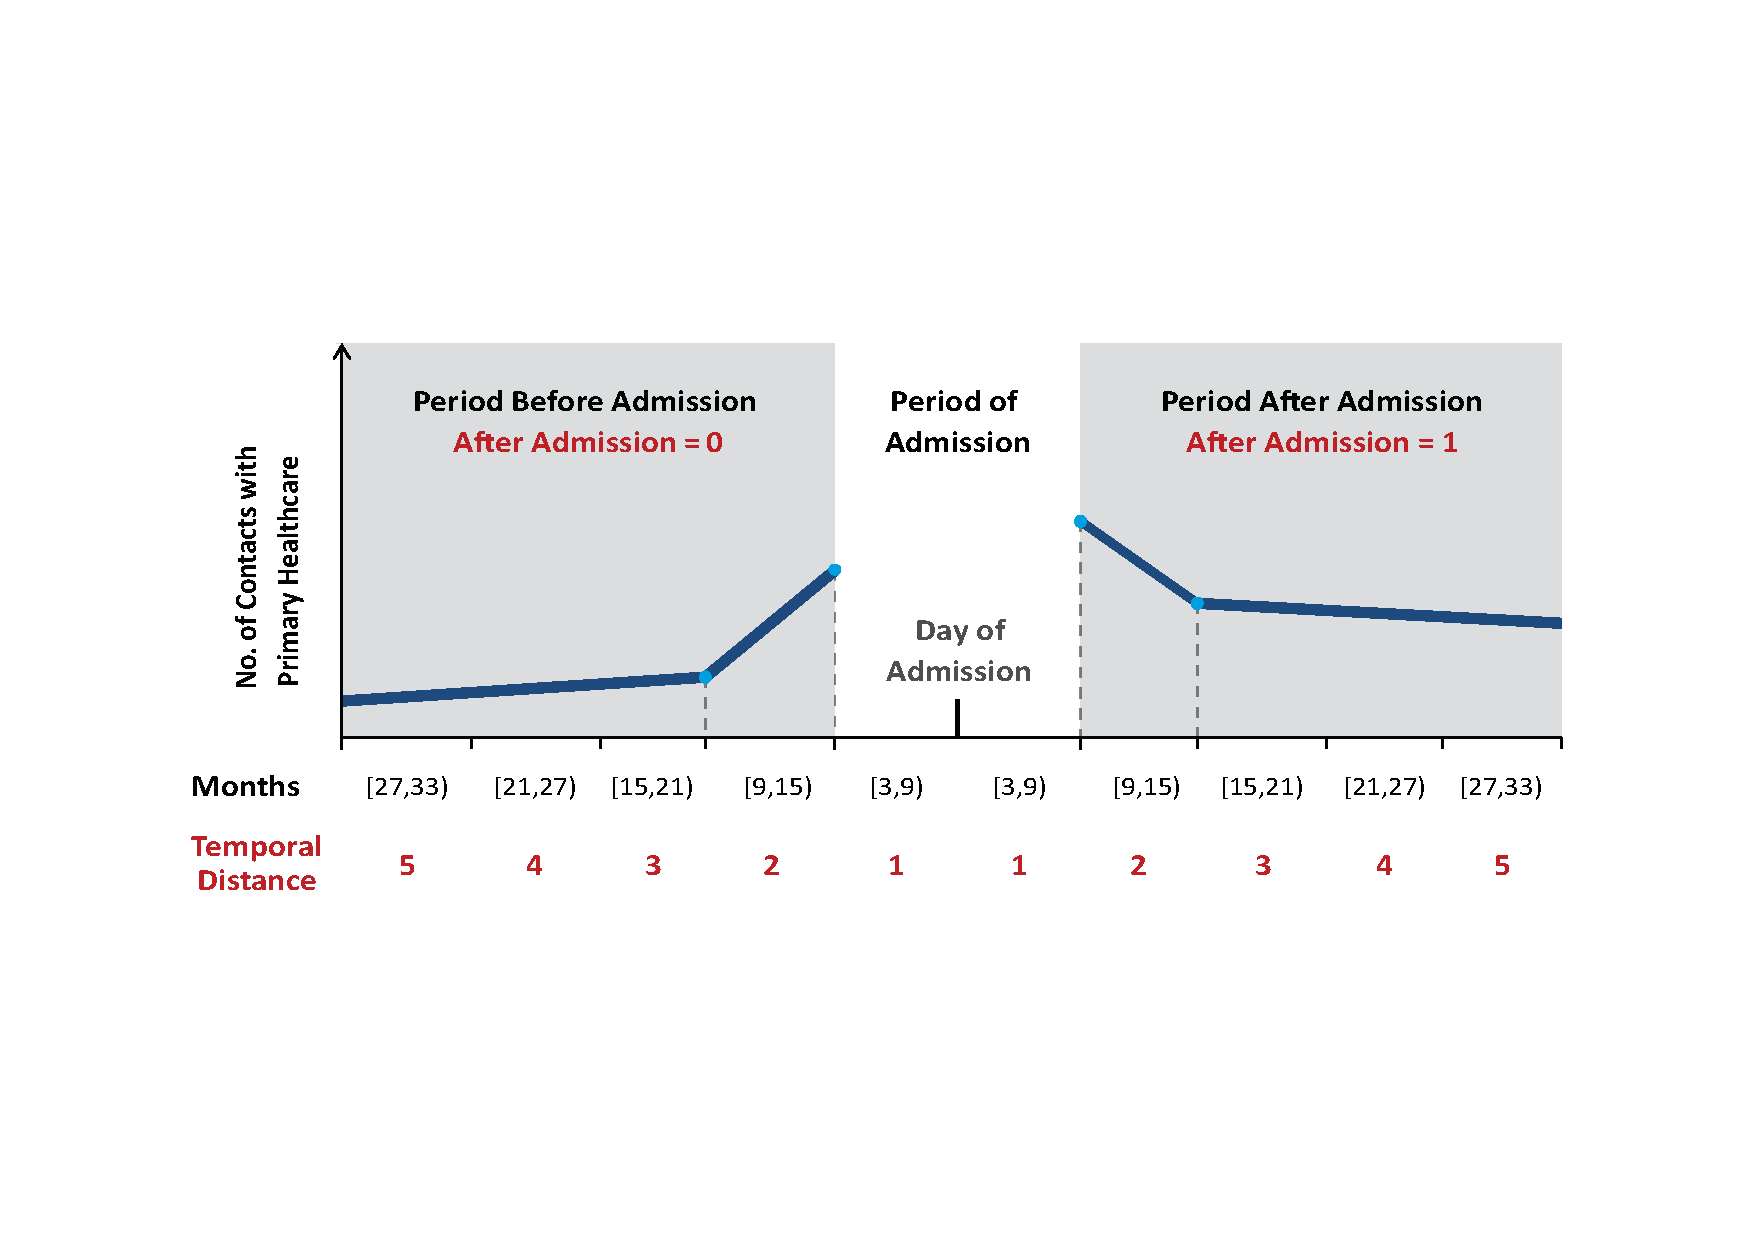
\includegraphics[scale=0.435]{Paper_4/MAIN_Figure_1.pdf}
		\caption*{\textbf{Figure 1:} Average number of days spent in hospital per person in 2014}
	\label{ch5:fig1}
	\end{figure}
	%--------------------%

\subsection{Changes in the Population Structure}

In 2014, the size of the Danish population was about 5.62 million. At that time, 
0.97 million individuals (17.3\%) were aged 0-14. The age group 15-49 consisted 
of 2.55 million individuals (45.4\%), while 1.43 million individuals (25.4\%) 
were aged 50-69. In 2014, 0.67 million Danes (11.9\%) were aged 70+, of whom 
0.29 million were men and 0.38 million were women.

Within the next decades, it is projected that the structure of the Danish population 
will change as the size of the population at older ages steadily increases. The 
projections up to 2050 are given in \hyperref[ch5:fig2]{Figure 2}. In 2050, it is forecast that the 
size of the Danish population will increase to 6.43 million. For the population 
younger than 70, only small changes in size are anticipated. By 2050, 1.05 million 
individuals (16.3\%) will be aged 0-14, 2.70 million individuals (42.0\%) will be 
aged 15-49, and 1.41 million individuals (21.9\%) will be of age 50-69. In contrast, 
major changes are expected in the older population. By 2050, it is projected that 
1.27 million Danes (19.8\%) will be aged 70 or older, of whom 0.59 million will 
be men and 0.68 million will be women. By this time, the size of the age group 70 
is forecast to have almost doubled in absolute terms.\\


	%-----------------------%
	\begin{figure}[H]
		\centering
		\includegraphics[scale=0.450]{Paper_4/MAIN_Figure_2.pdf}
		\caption*{	\textbf{Figure 2:} Projected changes in the structure of the Danish 
					population by sex between 2018 and 2050, based on publicly 
					available data provided by Statistics Denmark}
	\label{ch5:fig2}
	\end{figure}
	%-----------------------%


\subsection{Changes in Hospital Days}

In 2014, we observed 3.75 million hospital days in the Danish population. The 
population aged 0-14 accounted for 0.19 million days (5.0\%), the population aged 
15-49 0.66 million days (17.7\%), and the population aged 50-69 accounted for 1.29 
million days (34.5\%). In 2014, men and women aged 70+ contributed 0.77 and 0.85 
million hospital days respectively, together accounting for 42.9\% of all hospital 
days in that year.

We combined the age- and sex-specific hospital care use patterns of 2014 with 
Statistics Denmark's population projections to forecast the number of hospital 
days up to 2050. Results of the forecast are shown in \hyperref[ch5:fig3]{Figure 3}. 
The total number of hospital days per year is set to increase by 47\% within the observed 
period, reaching an overall level of 5.51 million days in 2050. The number of hospital 
days among the population younger than 70 is forecast to remain relatively stable 
during the projection period (Levels in 2050; 0-14: 0.21 million days (3.8\%) / 
15-49: 0.68 million days (12.7\%) / 50-69: 1.24 million days (22.5\%)). In contrast, 
the number of days accounted for by the population aged 70+ is projected to increase 
steadily and to more than double. By 2050, the population aged 70+ is forecast to 
account for 3.39 million days, or 61.4\% of all hospital days. Among the population 
aged 70+, men are expected to contribute 1.76 million days while women are expected 
to contribute 1.63 million days. This will correspond to 31.9\% and 29.5\%, respectively, 
of all hospital days in 2050.\\


	%-----------------------%
	\begin{figure}[H]
		\centering
		\includegraphics[scale=0.450]{Paper_4/MAIN_Figure_3.pdf}
		\caption*{	\textbf{Figure 3:} Projected annual number of hospital days until 2050}
	\label{ch5:fig3}
	\end{figure}
	%-----------------------%


\subsection{Sensitivity Analyses}

Our main findings do not include outpatient and obstetrics-related admissions. We 
examined the impact of these admissions on the age- and sex-specific patterns of 
health care use in 2014 and the projection of annual hospital days up to the year 
2050. We controlled separately for the impact of: (i) admissions due to childbearing 
and birth control, (ii) outpatient admissions, and (iii) a combination of both. 
Results of this robustness check (further discussed in \hyperref[ch5:textS1]{Supplementary Text S1}, and 
presented in \hyperref[ch5:figS1]{Supplementary Figure S1}, \hyperref[ch5:figS2]{Supplementary Figure S2}, 
and \hyperref[ch5:tabS2]{Supplementary Table S2} at the end of this paper) show 
similar trends and do not alter our conclusions. Irrespective of how we estimated 
the age- and sex-specific hospital care use in the baseline year 2014, the population 
aged 70+ remained the most important driver for the increasing amount of hospital 
days. In addition, men aged 70+ were always the fastest growing patient group treated 
in Danish hospitals in the period up to 2050. \\


%----------------------------------------------------------------%%----------------------------------------------------------------%


\section{Discussion}

In this study, we show the demographic profile of the demand for hospital 
care today and in the future. By keeping current age- and sex-specific patterns 
of hospital care use constant, we studied the changes attributable to population 
aging. Already today, the population aged 70+ accounts for half of all hospital 
days. We forecast that the absolute contribution of individuals aged 70+ to total 
hospital days will more than double and will account for nearly two thirds of all 
hospital days by 2050. By then, men aged 70+ are projected to be the largest 
patient group treated in Danish hospitals.\\
 
\subsection{Methodological Considerations}

We estimated the age- and sex-specific hospital care use patterns for the baseline 
year 2014 using routinely collected, individual-level register data. These data 
cover the total Danish population. Using register data eliminates recall biases, 
non-response and other problems regarding the under- or overstatement of healthcare 
use -- limitations which often affect studies based on self-reports.\citep{hunt2011women}

Forecasting is by its nature uncertain. This applies to two components of our 
projection: first, the structure of the Danish population and, second, patterns 
of hospital care use in the future. We used the most recent population projection 
of the Danish national statistical office. This projection is a deterministic 
projection and based on a continuation of current trends in fertility, mortality, 
and migration until the mid-21st century.\citep{denstat2018projection} Of all 
these parameters, future rates of migration are the most uncertain.\citep{de2010migration} 
Statistics Denmark assumes that in-migration will declines rapidly in the next 
few years, compared to the levels of 2015-2017, and will remain stable thereafter. 
We acknowledge that other projections do exist for Denmark, such as probabilistic 
projections by the United Nations.\citep{desa2017world} However, we decided to 
use the projections provided by Statistics  Denmark as they are the most recent 
and detailed for Denmark. 

Using a baseline forecast design, we froze the age- and sex-specific levels of hospital 
care use observed in 2014. Freezing rates assumes that age- and sex-specific patterns 
of hospital care use will remain constant in the future. Therefore, changes in the 
annual amounts of hospital days during the projection period are driven exclusively 
by changes in the demographic profile of the population. Keeping baseline levels 
constant during the projection period is a pragmatic approach in forecasting and 
has been applied to detailed projections of hospital care use\citep{vrhovec2016population} 
or fertility.\citep{bohk2018forecast} Especially when over-arching trends are 
difficult to predict, freezing rates has been shown to outperform statistically 
sophisticated techniques.\citep{bohk2018forecast} \\

\subsection{Health and Hospital Care Use in Aging Populations}

In line with previous findings, our study shows that hospital care use at late- 
and post-working ages is especially important for the total national hospital 
care demand. Previous research has shown that two opposite trends may have an 
impact on future hospital care use levels at these ages. On the one hand, the 
compression and postponement of morbidity may continue to reduce levels of hospital 
care use among the elderly.\citep{vaupel2010biodemography} Studies have shown 
that the incidences of leading causes of death, including stroke and MI, are 
consistently declining in low-mortality countries at all ages, including 
Denmark.\citep{schmidt201225} It has also been shown that cognitive functioning 
of the old and oldest-old has improved significantly within recent decades.\citep{christensen2013physical} 
Individuals of post-working age have been found to be increasingly happy 
and satisfied with their life considering the toll that aging generally 
takes on well-being, health and physical functioning.\citep{vestergaard2015physical}

On the other hand, it may be that the time spent with major chronic diseases 
does not shrink as life expectancy increases, and that frailty among the elderly 
even increases.\citep{clegg2013frailty} In addition, new medical technologies 
may contribute to increased treatment of this age group in hospitals, leading 
to higher levels of hospital care use in the future among the old and oldest 
old.\citep{oksuzyan2013changes} At the same time, these new technologies may 
enable a shift of treatments from inpatient to outpatient or primary healthcare 
settings. As both of these changes might have an impact at the same time, 
the general direction of population-level trends in hospital care use is difficult 
to predict. We therefore consider our findings to be neither overly optimistic -- 
nor pessimistic -- but to reflect a possible scenario.

Irrespective of long-term trends in age patterns and admission strategies, health 
behaviors impact population health and, as a consequence, future hospital care 
use. Studies show that smoking, hazardous drinking, obesity, lack of physical 
activity, and an unhealthy diet are associated with a higher risk of hospitalization 
at the individual level.\citep{hanlon2007analysis}  In Denmark, the general trend 
is towards healthier habits: smoking rates are decreasing, diet has improved, 
and physical inactivity has decreased.\citep{groth2014disparities} Future levels 
of hospital care use at the population level will be associated with the age pattern 
of diseases, trends in health behaviors within populations, as well as with the 
organizational structure and performance of healthcare systems. \\

\subsection{Implications of a Changing Patient Profile}

We forecast that the number of hospital days for individuals aged 70+ will almost 
double in the period up to 2050, as an increasing number of individuals reache 
older ages. The reason for this is rather simple: older individuals, on average, 
spend more days in hospital than younger individuals. Age is a major risk factor 
for non-communicable diseases and therefore directly linked with hospital care use 
levels.

Studies have shown that the prevalence of most leading causes of admission is 
likely to increase as the population ages, including circulatory diseases and 
cancers.\citep{christensen2009ageing} While more individuals survive to older 
ages, and better treatment of diseases reduces case fatality, the number of 
individuals at older ages with chronic conditions, complex diseases and multi-morbidity 
is increasing.\citep{christensen2009ageing} In the light of these findings, 
inadequacies in geriatric training for the medical workforce have to be addressed 
in order to meet the complex needs of older patients; this will involve changes 
in curricula, the role of senior staff, and the organizational structure of 
hospitals.\citep{samra2015medical} Addressing these deficiencies may encourage 
medical students and student nurses to join the field of geriatrics, and contribute 
to better treatment of the elderly.\citep{fisher2018pejorative} The education 
of healthcare workers is a long-term process and requires responsible and careful 
planning. Preparing healthcare services for changing needs requires an understanding 
of who the future patients will be. To meet future hospital care needs, reducing 
prejudice towards the elderly among medical students and student nurses has to be 
given special emphasis -- as soon as possible.\citep{fisher2018pejorative} Only 
sufficient numbers, and a well-balanced mix of specialists and sub-specialists, 
can ensure that the healthcare challenges of aging populations will be met in 
the coming decades.\citep{dall2013aging} \\

\subsection{Conclusion}

Already today, individuals of post-working age are the largest patient group 
in hospital settings. As populations age, the share of these age groups is 
projected to steadily increase. To ensure that hospitals meet the needs of 
future patients, a variety of responses are necessary. Reducing negative 
stereotypes and creating incentives to work with the elderly has to be one 
first step in order to ensure that future doctors and nurses are motivated 
and qualified to join the field of geriatrics. Taking into account the time 
frame to train medical staff, these issues should be addressed sooner rather 
than later. 


%----------------------------------------------------------------%%----------------------------------------------------------------%


\newpage


\section{Supplementary Material}
%%% Supplementary Text S1 %%%


\newpage


\begin{landscape}

%%% Supplementary Table S1 %%%
\begin{table}[H]
\scriptsize
\centering
\caption*{\textbf{Supplementary Table S1:} Overview on projection assumptions.}
\medskip
\begin{tabular}{llll}
\hline
\textbf{Process} & \textbf{Parameters}        & \textbf{(Sub-) Population} & \textbf{Value}                 
\\
\hline
                   &                         &                                                               &                         \\
\textbf{\textit{Mortality}}          & e(0) in 2059            & Men                                                           & 87.1 years              \\
                   & (Lee-Carter Method)     & Women                                                         & 89.5 years              \\
                   &                         &                                                               &                         \\
\textbf{\textit{Fertility}}          & Long-Term TFR           & Danish Origin - Danish Citizenship                            & 1.91                    \\
                   &                         & Danish Origin - foreign Citizenship                           & 1.91                    \\
                   &                         & Immigrants non-Western countries - Danish citizenship:        & 1.68                    \\
                   &                         & Immigrants non-Western countries - foreign citizenship:       & 1.97                    \\
                   &                         & Immigrants Western countries - Danish citizenship:            & 1.61                    \\
                   &                         & Immigrants Western countries - foreign citizenship:           & 1.77                    \\
                   &                         & Descendants from non-Western countries - Danish citizenship:  & 1.91                    \\
                   &                         & Descendants from non-Western countries - foreign citizenship: & 1.91                    \\
                   &                         & Descendants from Western countries - Danish citizenship:      & 1.75                    \\
                   &                         & Descendants from Western countries - foreign citizenship:     & 1.75                    \\
                   &                         &                                                               &                         \\
                   & Origin at birth         & Danish origin - Danish citizenship                            & 100.00                  \\
                   & (frequencies of change) & Danish origin - foreign citizenship                           & 100.00                  \\
                   &                         & Immigrants from non-Western countries - Danish citizenship    & 24.50                   \\
                   &                         & Immigrants from non-Western countries - foreign citizenship   & 21.80                   \\
                   &                         & Immigrants from Western countries - Danish citizenship        & 73.10                   \\
                   &                         & Immigrants from Western countries - foreign citizenship       & 36.40                   \\
                   &                         & Descendants from non-Western countries - Danish citizenship   & 100.00                  \\
                   &                         & Descendants from non-Western countries - foreign citizenship  & 41.40                   \\
                   &                         & Descendants from Western countries - Danish citizenship       & 100.00                  \\
                   &                         & Descendants from Western countries - foreign citizenship      & 66.30                   \\
                   &                         &                                                               &                         \\
\textbf{\textit{Out-Migration}}      & Number of out-migrants  & entire Danish population and all groups of origin             & N/A                     \\
                   &                         &                                                               & (not specified  \\
                   &                         &                                                               & as 2015--2017)   \\
                   &                         &                                                               &                         \\
\textbf{\textit{In-Migration}}       & Number of in-migrants   & Immigrants without Danish citizenship                         & 17,000                  \\
                   &                         & Western immigrants without Danish citizenship                 & 28,100                  \\
                   &                         & Reimmigration: Danish origin and all with Danish citizenship  & N/A                     \\
                   &                         &                                                               & (not  specified, \\
                   &                         &                                                               &  as 2015--2017)   \\ \hhline{====}
\end{tabular}
\label{ch5:tabS1}
\end{table}


\end{landscape}


%----------------------------------------------------------------%%----------------------------------------------------------------%


\newpage

\textbf{Supplementary Text S1:} Further Remarks on Sensitivity Analyses.\\

Our main findings do not consider outpatient admissions and obstetrics-related 
admissions \textbf{(Setting A)}. We investigated the impact of obstetrics-related 
admissions \textbf{(Setting B)}. We specified this category as O.00 -- O.99 and 
Z.30 -- Z.39 using the International Classification of Diseases (ICD), 10th Revision. In addition, 
we estimated the contribution of those outpatient treatments, which were provided 
within hospitals \textbf{(Setting C)}. Each outpatient treatment was approximated to contribute 
exactly one day. We used this approximation for outpatient admissions since the 
registers provide neither the exact number of days an outpatient has spent in the 
hospital, nor an overview of the provided services. Instead, the information in 
the registers on outpatient treatments covers the start and the end date of the 
treatment period for administrative purposes. We further studied the combined impact 
of outpatient treatments and obstetrics-related admissions \textbf{(Setting D)}.

\label{ch5:textS1}

While \hyperref[ch5:figS1]{Supplementary Figure S1} compares age- and sex-specific 
trajectories for the baseline year 2014 reflecting these four settings, 
\hyperref[ch5:figS2]{Supplementary Figure S2} compares the results of the 
corresponding projections. A summary of projection results for all four settings 
is presented in \hyperref[ch5:tabS2]{Supplementary Table S2}.\\


%----------------------------------------------------------------%%----------------------------------------------------------------%


%%% Supplementary Figure S1 %%%


\newpage


	%------------------%
	\begin{figure}[H]
		\centering
		\includegraphics[scale=0.45]{Paper_4/Supplementary_Figure_S1.pdf}
		\caption*{	\textbf{Supplementary Figure S1:} Average number of days spend 
					in hospital per person in 2014 by age and for different 
					admission types and causes.}
	\label{ch5:figS1}
	\end{figure}
	%--------------------%
	

%----------------------------------------------------------------%%----------------------------------------------------------------%


%%% Supplementary Figure S2 %%%


\newpage


	%------------------%
	\begin{figure}[H]
		\centering
		\includegraphics[scale=0.45]{Paper_4/Supplementary_Figure_S2.pdf}
		\caption*{	\textbf{Supplementary Figure S2:} Projected annual number of hospital 
					days up to the year 2050 for different admission types and causes.}
	\label{ch5:figS2}
	\end{figure}
	%--------------------%


%----------------------------------------------------------------%%----------------------------------------------------------------%


%%% Supplementary Table S2 %%%

\begin{landscape}



%%% PART I %%%
\begin{table}[htbp]
  \centering
  \caption*{	\textbf{Supplementary Table S2:} Comparing the impact of different 
  				specifications of hospital care use for 2014 (baseline year) and 
  				2050 (last year of the projection period).}
    \begin{tabular}{c|cc|cc|cc|cc}
    \toprule
    \multicolumn{9}{c}{\textbf{2014  - Men}} \\
    \midrule
    \textbf{Age} & \multicolumn{2}{c|}{\textbf{(A) Days in Hospital}} & \multicolumn{2}{c|}{\textbf{(B) Days in Hospital}} & \multicolumn{2}{c|}{\textbf{(C) Days in Hospital}} & \multicolumn{2}{c}{\textbf{(D) Days in Hospital}} \\
    \textbf{Group} & \textbf{N in Mio.} & \textbf{Share in \%} & \textbf{N in Mio.} & \textbf{Share in \%} & \textbf{N in Mio.} & \textbf{Share in \%} & \textbf{N in Mio.} & \textbf{Share in \%} \\
    \midrule
    0-14  & 0.10   & 2.66   & 0.10   & 2.51   & 0.33   &  4.14   &  0.33   &  4.03 \\
    15-49 & 0.31   & 8.31   & 0.31   & 7.84   & 0.95   &  11.88  &  0.95   & 11.48 \\
    50-69 & 0.72   & 19.30  & 0.72   & 18.19  & 1.30   &  16.33  &  1.30   & 15.73 \\
    70+   & 0.77   & 20.50  & 0.77   & 19.32  & 1.14   &  14.34  &  1.14   & 13.81 \\
    \midrule
    \textbf{All } & \textbf{1.90} & \textbf{50.77} & \textbf{1.90} & \textbf{47.86} & \textbf{3.72} & \textbf{46.69} & \textbf{3.72} & \textbf{45.05} \\
    \midrule
    \multicolumn{9}{c}{\textbf{2014  - Women}} \\
    \midrule
    \textbf{Age } & \multicolumn{2}{c|}{\textbf{(A) Days in Hospital}} & \multicolumn{2}{c|}{\textbf{(B) Days in Hospital}} & \multicolumn{2}{c|}{\textbf{(C) Days in Hospital}} & \multicolumn{2}{c}{\textbf{(D) Days in Hospital}} \\
    \textbf{Group} & \textbf{N in Mio.} & \textbf{Share in \%} & \textbf{N in Mio.} & \textbf{Share in \%} & \textbf{N in Mio.} & \textbf{Share in \%} & \textbf{N in Mio.} & \textbf{Share in \%} \\
    \midrule
    0-14  & 0.09  & 2.31  & 0.09  & 2.18  & 0.29  & 3.60  & 0.29  & 3.47 \\
    15-49 & 0.35  & 9.34  & 0.53  & 13.42 & 1.14  & 14.31 & 1.44  & 17.38 \\
    50-69 & 0.57  & 15.18 & 0.57  & 14.31 & 1.51  & 18.92 & 1.51  & 18.23 \\
    70+   & 0.84  & 22.41 & 0.88  & 22.23 & 1.31  & 16.47 & 1.31  & 15.87 \\
    \midrule
    \textbf{All } & \textbf{1.85} & \textbf{49.23} & \textbf{2.07} & \textbf{52.14} & \textbf{4.24} & \textbf{53.31} & \textbf{4.54} & \textbf{54.95} \\
    \midrule
    \textbf{Total} & \textbf{3.75} & \textbf{100} & \textbf{3.98} & \textbf{100} & \textbf{7.96} & \textbf{100} & \textbf{8.26} & \textbf{100} \\
    \bottomrule
    \bottomrule
    \end{tabular}%
\label{ch5:tabS2}
\end{table}%

  

%%% PART II %%%

\begin{table}[htbp]
  \centering
  \caption*{	\textbf{Supplementary Table S2 - Continued:} Comparing the impact of different 
  				specifications of hospital care use for 2014 (baseline year) and 
  				2050 (last year of the projection period).}
    \begin{tabular}{c|cc|cc|cc|cc}
    \toprule
    \multicolumn{9}{c}{\textbf{2050  - Men}} \\
    \midrule
    \textbf{Age} & \multicolumn{2}{c|}{\textbf{(A) Days in Hospital}} & \multicolumn{2}{c|}{\textbf{(B) Days in Hospital}} & \multicolumn{2}{c|}{\textbf{(C) Days in Hospital}} & \multicolumn{2}{c}{\textbf{(D) Days in Hospital}} \\
    \textbf{Group} & \textbf{N in Mio.} & \textbf{Share in \%} & \textbf{N in Mio.} & \textbf{Share in \%} & \textbf{N in Mio.} & \textbf{Share in \%} & \textbf{N in Mio.} & \textbf{Share in \%} \\
    \midrule
    0-14  & 0.11  & 2.03  & 0.11  & 1.96  & 0.37  & 3.45  & 0.37  & 3.35 \\
    15-49 & 0.32  & 5.83  & 0.32  & 5.62  & 0.99  & 9.38  & 0.99  & 9.11 \\
    50-69 & 0.69  & 12.54 & 0.69  & 12.08 & 1.25  & 11.83 & 1.25  & 11.46 \\
    70+   & 1.76  & 31.88 & 1.76  & 30.72 & 2.54  & 23.99 & 2.54  & 23.25 \\
    \midrule
    \textbf{All } & \textbf{2.88} & \textbf{52.28} & \textbf{2.88} & \textbf{50.38} & \textbf{5.14} & \textbf{48.65} & \textbf{5.15} & \textbf{47.17} \\
    \midrule
    \multicolumn{9}{c}{\textbf{2050  - Women}} \\
    \midrule
    \textbf{Age } & \multicolumn{2}{c|}{\textbf{(A) Days in Hospital}} & \multicolumn{2}{c|}{\textbf{(B) Days in Hospital}} & \multicolumn{2}{c|}{\textbf{(C) Days in Hospital}} & \multicolumn{2}{c}{\textbf{(D) Days in Hospital}} \\
    \textbf{Group} & \textbf{N in Mio.} & \textbf{Share in \%} & \textbf{N in Mio.} & \textbf{Share in \%} & \textbf{N in Mio.} & \textbf{Share in \%} & \textbf{N in Mio.} & \textbf{Share in \%} \\
    \midrule
    0-14  & 0.10   & 1.75  & 0.10   & 1.69  & 0.32  & 2.99  & 0.32  & 2.90 \\
    15-49 & 0.36   & 6.53  & 0.57   & 9.92  & 1.18  & 11.16 & 1.51  & 13.88 \\
    50-69 & 0.55   & 9.93  & 0.55   & 9.57  & 1.47  & 13.86 & 1.47  & 13.43 \\
    70+   & 1.63   & 29.51 & 1.63   & 28.44 & 2.47  & 23.35 & 2.47  & 22.62 \\
    \midrule
    \textbf{All } & \textbf{2.63} & \textbf{47.72} & \textbf{2.84} & \textbf{49.62} & \textbf{5.43} & \textbf{51.35} & \textbf{5.76} & \textbf{52.83} \\
    \midrule
    \textbf{Total} & \textbf{5.51} & \textbf{100} & \textbf{5.72} & \textbf{100} & \textbf{10.57} & \textbf{100} & \textbf{10.91} & \textbf{100} \\
    \bottomrule
    \bottomrule
    \end{tabular}%
\end{table}%

\end{landscape}
